% TFF-Title: EPC query-rake acknowledgement cycle
% TFF-Family: flowchart
% TFF-Tags: flowchart, epc, state-machine, retry-loop, orthogonal-routing
% TFF-Description: EPC processing chain with a clean top-level retry route and separated process annotations.
% TFF-Origin: https://texample.net/epc-flow-charts/
% TFF-License: CC BY-SA 4.0
% TFF-Attribution: Adapted from Fabian Schuh's EPC flow charts example on TeXample.net
\documentclass[tikz,border=8pt]{standalone}
\usetikzlibrary{arrows.meta,positioning}
\begin{document}
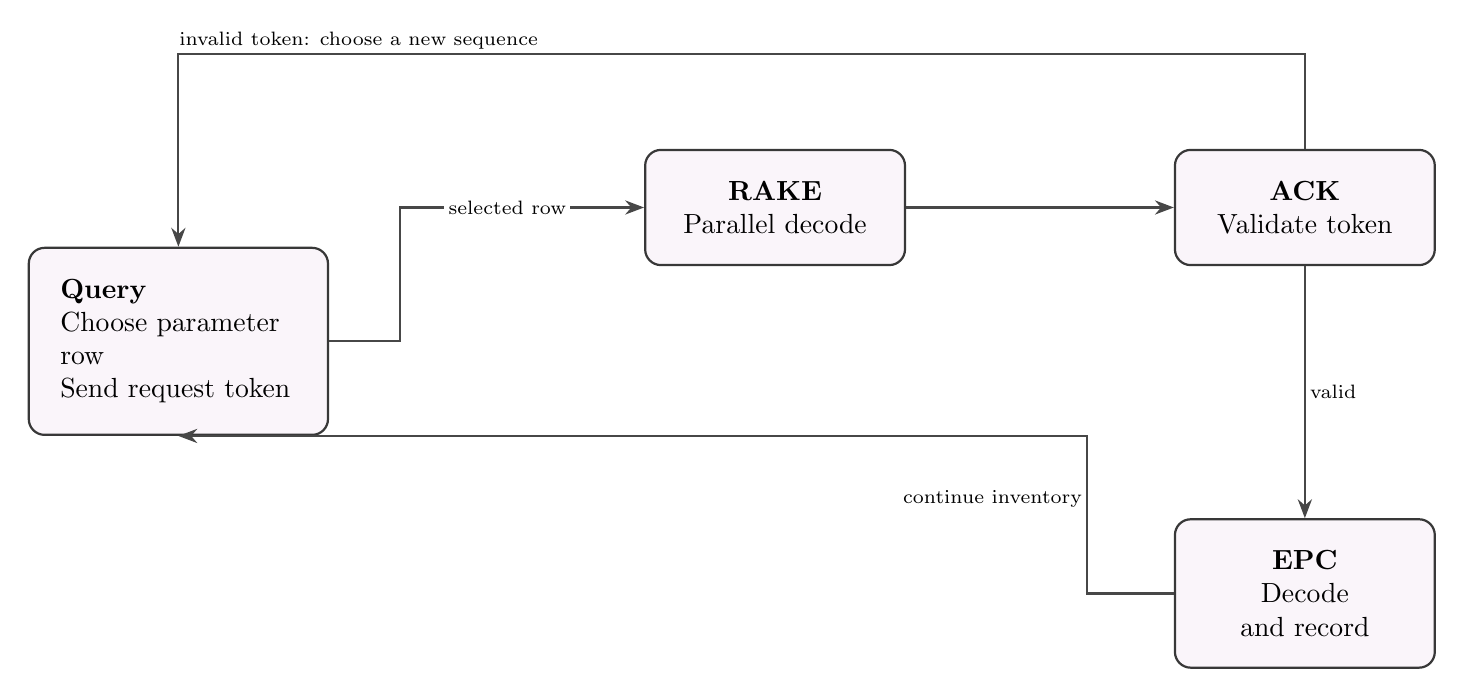
\begin{tikzpicture}[
  state/.style={rounded corners=2mm,draw=black!78,line width=.8pt,
    fill=violet!4,minimum height=12mm,text width=30mm,align=left,inner sep=4mm},
  smallstate/.style={state,text width=25mm,align=center},
  flow/.style={-{Stealth[length=2.4mm]},draw=black!72,line width=.8pt},
  labelbox/.style={fill=white,inner sep=1.5pt,font=\scriptsize,align=center}
]
\node[state] (query) {\textbf{Query}\\Choose parameter row\\Send request token};
\node[smallstate,right=40mm of query,yshift=17mm] (rake) {\textbf{RAKE}\\Parallel decode};
\node[smallstate,right=34mm of rake] (ack) {\textbf{ACK}\\Validate token};
\node[smallstate,below=32mm of ack] (epc) {\textbf{EPC}\\Decode and record};
\draw[flow] (query.east) -- ++(9mm,0) |- node[labelbox,pos=.72] {selected row} (rake.west);
\draw[flow] (rake.east) -- (ack.west);
\draw[flow] (ack.south) -- node[labelbox,right] {valid} (epc.north);
\draw[flow] (ack.north) -- ++(0,12mm) -|
  node[labelbox,pos=.42,above] {invalid token: choose a new sequence}
  (query.north);
\draw[flow] (epc.west) -- ++(-11mm,0) |-
  node[labelbox,pos=.30,left] {continue inventory}
  (query.south);
\end{tikzpicture}
\end{document}
